Consider the following PD feedback control system
\begin{center}
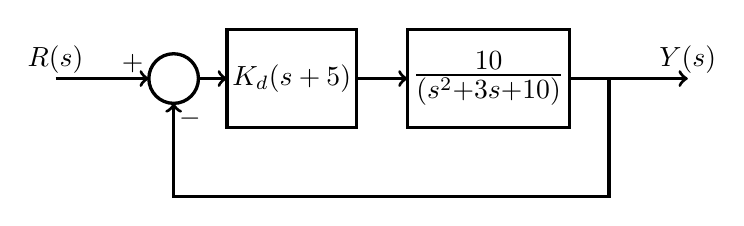
\begin{tikzpicture}[scale=1,inner sep=0pt,outer sep=0pt,very thick,
sysblock/.style={draw,rectangle,inner sep=2pt,minimum width=1.25cm,minimum height=1.25cm,very thick}]
\draw (2,0) node[draw,circle] (sum1) {$\rule{0pt}{18pt}$};
\draw (3.5,0) node[sysblock] (K) {$K_d (s+5)$};
\draw (6,0) node[sysblock] (G) {\Large $\frac{10}{(s^2+3s+10)}$};
\draw[->] (.5,0) node[above=2pt] {$R(s)$} -- (sum1.180) node[above left=2pt] {$+$};
\draw[->] (sum1.0) --  (K);
\draw[->] (K) -- (G);
\draw[->] (G.0) -- ++(1.5,0) node[above=2pt] {$Y(s)$};
\draw[->] (G.0) ++(0.5,0) -- ++(0,-1.5) -| (sum1.-90) node[below right=2pt] {$-$};
\end{tikzpicture}
\end{center}
\begin{enumerate}[(a)]
\item Import $G(s)$ into \textsc{Matlab}'s \texttt{sisotool}.
\item Go to \texttt{File --> Toolbox Preferences --> SISO Tool} and click the button for the Zero/pole/gain format.
\item Within the \texttt{Control and Estimation Tools Manager}, select \texttt{Compensator Editor} and add a real zero at $-5$ by right clicking in the \texttt{Dynamics} box.
\item You will now see a root locus for your closed-loop system. To see the closed-loop step response, click \texttt{Analysis --> Response to Step Command}.
\item Drag the closed-loop poles (pink squares) along the loci until you feel you have reached an ``optimal'' closed-loop transient response, i.e., a small \%OS and fast rise time and settling time. 
\item Submit your final controller $C(s)$ and the plot of your closed-loop step response.
\end{enumerate}